\documentclass[10pt]{article}
\usepackage[margin=.65in]{geometry}
\usepackage{graphicx,booktabs,hyperref,amsmath,amssymb,array}
\hypersetup{colorlinks=true,urlcolor=blue}
\setlength{\parindent}{0pt}
\setlength{\parskip}{5pt}
\begin{document}
\begin{center}
{\Large A twist point enables a pairing transfer}\\[4pt]
{\large A checked finite route to finite-field index calculus}\\[4pt]
24 October 2026 $\cdot$ \texttt{pairing-20261024T0442Z} $\cdot$ PR \#2381
\end{center}
\textbf{Request and result.} Pursue the positive pairing connection rather
than a universal no-connection claim. In the retained $\mathbb F_{43}$ example,
Lean checks the explicit Miller function on actual elliptic points, all
121 generator pairs, and exact logarithm transport. Native finite-field index
calculus recovers all eleven scalar logs, independently verified in Rust.
The complete auxiliary-point census below checks when this route is nontrivial
and when it degenerates. No speed or general hardness claim is made.

Let $E/\mathbb F_{43}:y^2=x^3+x$, $r=11$, $P=(31,18)$ and $Q=(13,24)=7P$.
For $d=2$, the monic twist is $E_d:Y^2=X^3+4X$. In
$K=\mathbb F_{43}[u]/(u^2-2)$, the point $T=(35,12)$ maps to
$S=(39,3u)$ by $\psi(X,Y)=(X/2,Y/(2u))$. The explicit formula yields
\[
g=e(P,S)=2+25u,\quad h=e(Q,S)=11+19u=g^7,\quad g^{11}=1,\quad g\ne1.
\]
The target is norm one: $g^{43}g=1$. The eleven powers of $g$ are distinct.

\begin{center}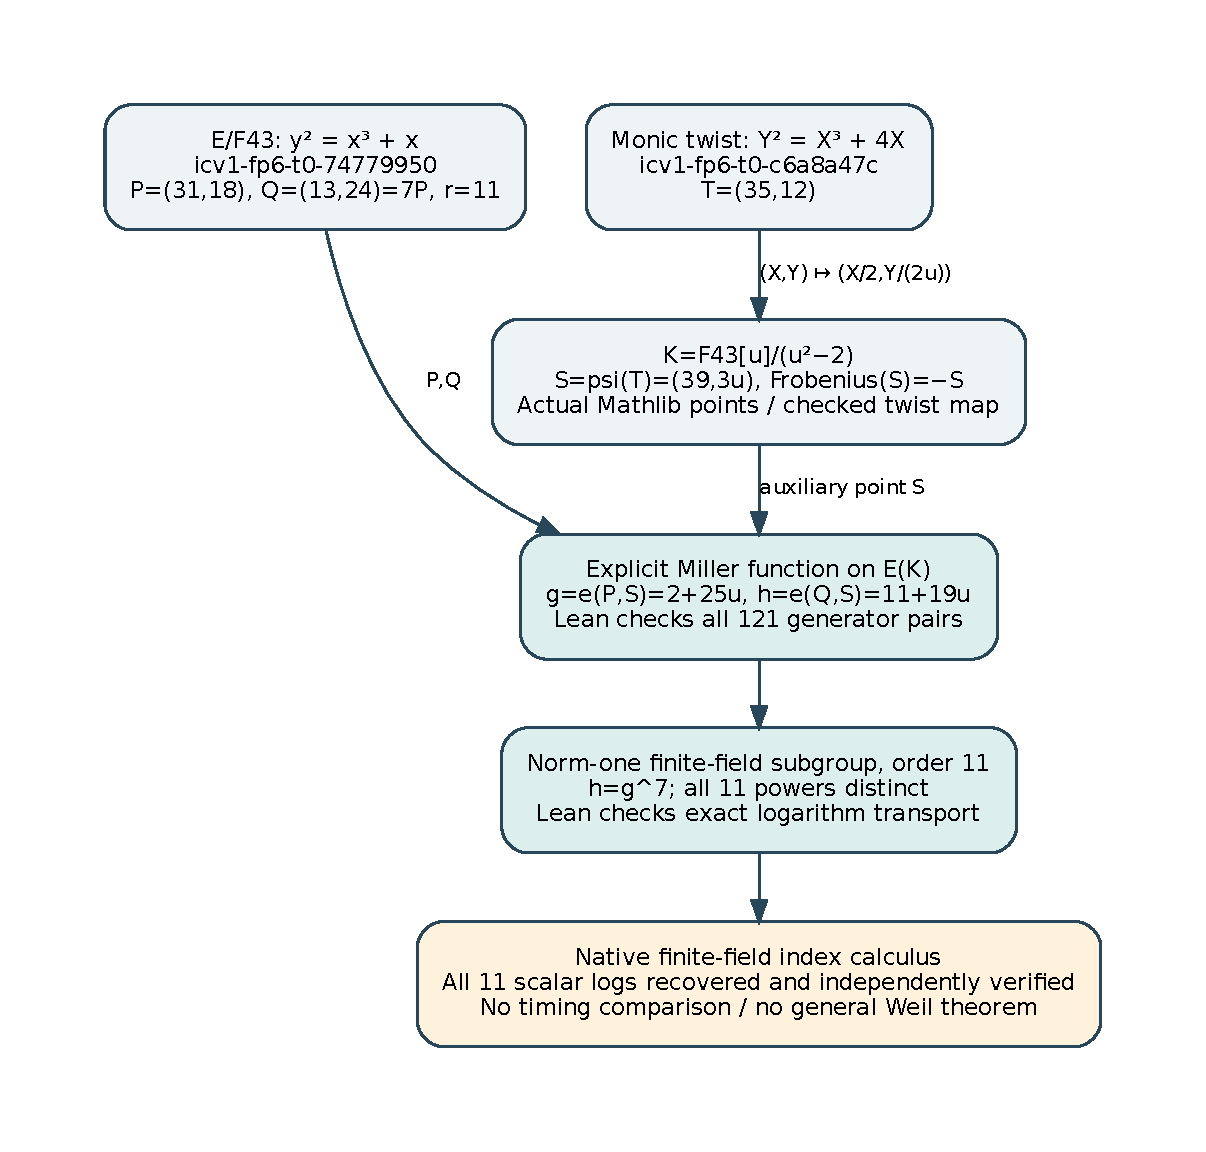
\includegraphics[height=4.65in,width=\linewidth,keepaspectratio]{bridge.pdf}\end{center}
\small Full exact model/subgroup identifiers and source records are in the
accompanying \path{README.md}; no model or representation is added by this round.
The direct odd-order mixed-relation obstruction remains valid and does not
rule out this pairing route.\normalsize

\newpage
\begin{center}{\Large Complete finite auxiliary-point census}\end{center}
\textbf{Frozen protocol.} Commit \texttt{dcd89832fc6169dd71dad048cc59a70f694a66bc}
preceded execution. Every nonsingular short model over
$p\in\{5,7,11,13,17,19\}$ is included: 942 models. The least positive nonsquare
$d$ defines the monic twist $Y^2=X^3+d^2aX+d^3b$. Every odd prime divisor $r$
of the enumerated rational order is retained. The 649 nonshared-prime cases
have no nonzero rational twist $r$-torsion. The $p=43$ example is additional.

For each of 274 shared-prime cases, $P$ is the first nonzero rational cofactor
projection. For every rational twist point $T$, compute
$S=\psi([\#E_d/r]T)$. Both implementations check its actual curve equation,
$[r]S=O$, Frobenius negation, pairing value, target order and norm one.

\begin{center}
\begin{tabular}{rrrrr}
\toprule
$r$ & Shared cases & Auxiliary points & Zero images & Nonzero images\\\midrule
3 & 186 & 2,952 & 984 & 1,968\\
5 & 72 & 1,440 & 288 & 1,152\\
7 & 16 & 224 & 32 & 192\\\midrule
Total & 274 & 4,616 & 1,304 & 3,312\\\bottomrule
\end{tabular}
\end{center}
All zero images pair to one. All nonzero images give nontrivial order-$r$
values. Each shared case attains all $r$ target values. Counts include repeated
images from different auxiliary sources; they are not independent relation counts.

\begin{center}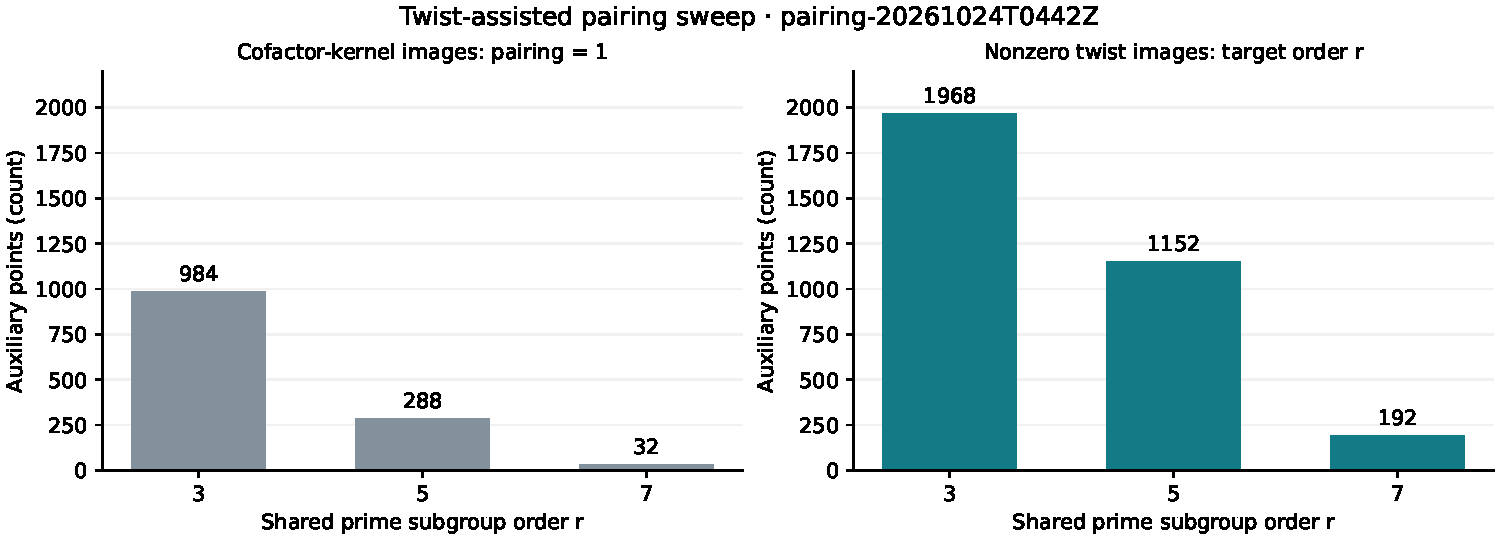
\includegraphics[width=\linewidth]{auxiliaries.pdf}\end{center}
\small Exact exhaustive counts recorded by the independent auditor, run
\texttt{pairing-20261024T0442Z}. Units: auxiliary points; no sampling uncertainty
or timing measurement. Graph data is copied from \path{native/pairing-20261024T0442Z/audit.json}.
Python performs presentation only.\normalsize

\textbf{Applicability restriction.} Shared odd $r$ divides $N$ and $N_t$, and
$N+N_t=2(p+1)$, hence $p=-1\pmod r$. Since $r$ is odd, $p\ne1\pmod r$:
the embedding degree is two. This is checked in every shared case and is
consistent with the retained Lean arithmetic implications. A quadratic twist
alone does not give small embedding degree for an arbitrary target subgroup.

\textbf{Independent arithmetic.} C++17 uses the existing packed-field curve
backend and a binary Miller chain. Rust independently enumerates coefficient
pairs, inverts by exponentiation, and uses a linear Miller chain. It checks
every point, cofactor image, Frobenius sign, shifted/direct value and first
legal offset. Field and curve arithmetic are not shared. The replay caps
are 600 seconds each; neither was reached. No timing or fastest-tool claim follows.

\newpage
\begin{center}{\Large Kernel checks and controls}\end{center}
\textbf{Concrete finite transfer.} \path{lean/PairingFixture.lean} constructs
the actual Mathlib nonsingular points over the computable field
$\operatorname{QuadraticAlgebra}(\mathbb Z/43\mathbb Z,2,0)$. It checks
the twist source, $[7]P=Q$, $[11]P=[11]S=O$, the two Frobenius signs, and
the explicit Miller values. The function uses line functions and a linear
addition chain, with support collisions represented by \texttt{none}.
It is not defined using a discrete-log lookup. Kernel evaluation proves
\[
\forall a,b\in\{0,\ldots,10\},\quad
\operatorname{weil11}([a]P,[b]S)=\operatorname{some}(g^{ab}).
\]
The distinct-power theorem then proves
\[
\operatorname{weil11}([a]P,S)=\operatorname{some}(g^b)\ \Longleftrightarrow\ a=b.
\]
This is a finite actual-function reduction. It does not prove universal
equality with a separately defined geometric divisor pairing.

\textbf{General conditional implication.} \path{lean/PairingTransfer.lean}
proves scalar compatibility and exact prime image order for a specified
additive-to-multiplicative homomorphism with nontrivial generator image.
It proves unique exponent recovery under those explicit hypotheses. Generic
Weil bilinearity and nondegeneracy are not silently assumed to be discharged.
The norm multiplication polynomial is checked over every commutative ring:
\[
(xs+dyt)^2-d(xt+ys)^2=(x^2-dy^2)(s^2-dt^2).
\]
Native certificate \texttt{IDC1h23c0696a12358b08} binds the exact Lean source,
replays 32+16 points and rejects both false-plus-one and false-source controls.
It certifies only the polynomial, not the entire pairing theory.

\textbf{Axiom audit.} The two modules add 19 named theorems: 15 concrete
fixture statements and four character/norm statements. The unmodified scoped
gate passes \textbf{68 named research theorems / 85 audited declarations},
including 17 generated helpers, with zero failing or extra trusted native axioms.
Only \texttt{propext}, \texttt{Classical.choice} and \texttt{Quot.sound} occur.
Lean4.34.1 and Mathlib \texttt{d13f23b723b8a846827a245b89c10fc7d3f11612}
remain pinned. \texttt{lean4checker} is unavailable; no separate replay is claimed.

\textbf{Degeneracy and invalid-record controls.}
\begin{itemize}
\item All 274 same-source subgroup controls yield one using shifted disjoint
divisors. Direct evaluation is undefined in all 274 cases; undefined is not
treated as one. The first legal lexicographic offset is saved and reproduced.
\item Wrong-subgroup points exist in 270 cases and fail the $r$-torsion
precondition; four cases have no such point and retain explicit null controls.
Every point used remains on the correct nonsingular curve.
\item False pairing value, missing model, false summary count and false IC
coefficient payloads each cause exit101 and no audit receipt. Exact payloads,
hashes and diagnostics are retained.
\end{itemize}
All eleven native IC certificates have independently checked projected
factor-base logs, six-dimensional relation rank, target exponentiation and
actual source scalar. Producer random-search attempt counters are not an
independently rerun search. The IC algorithm itself is not formalized in Lean.

\newpage
\begin{center}{\Large Evidence, validation and remaining work}\end{center}
\begin{tabular}{p{.38\linewidth}p{.57\linewidth}}
\toprule
Requirement & Actual outcome\\\midrule
Full native sweep & 942 models, 274 shared cases, 4,616 auxiliary points; independent arithmetic replay passes\\
F43 positive fixture & All 121 generator pairs kernel-checked; all eleven IC logs independently verified\\
Unchanged study proof gate & PASS: 85 declarations, zero failing/trusted\\
Source-bound norm identity & Exact bytes, 32+16 replay points, false identity/source controls pass\\
Isolated native backend & 22 passed, zero failed/ignored\\
Fresh release library suite & 4,479 passed, zero failed, 119 existing ignores\\
Workflow metadata parser & Four tests passed; shell syntax checked\\
Frozen prior evidence & Unchanged; all failed attempts and source snapshots retained\\
Shared Conductor & Exit127; no task reservation or local replacement claimed\\
Merge & Held for conflicts, exact-head CI/access/review and completion gates\\\bottomrule
\end{tabular}

\textbf{What this establishes.} A real finite twist-assisted pairing route
to a finite-field logarithm exists in the explicit F43 example, and the native
IC solver recovers all scalar values. In the registered small-field population,
cofactor-zero, same-source and wrong-subgroup controls expose concrete
degeneracy/precondition failures. The direct mixed-relation obstruction and
this positive pairing connection concern different mechanisms.

\textbf{What remains.} General geometric pairing correctness/nondegeneracy
and a uniform reduction remain open. So do general-model normalization,
exceptional S3/S4 lifting and universal trace-zero geometry in the existing
problem record. No practical/asymptotic IC advantage, general hardness result,
GHS claim or invalid-curve attack is supplied. A next pairing experiment should
preregister denominator-safe evaluation on non-k2 subgroup families and price
the destination solver before an advantage claim. That experiment is not running.

\textbf{Reproduction.} From the repository root, run
\begin{verbatim}
bash research/quadratic_twist_evidence_20261021/run-pairing.sh \
  /tmp/twist-pairing-fresh
tools/lean/proof-gate.sh --out /tmp/twist-pairing-proof \
  research/quadratic_twist_evidence_20261021/lean
\end{verbatim}
The first command checks full native results, independent audit, exact frozen
bytes, certificates, corruptions and backend tests. The second builds and
audits all seven Lean modules. Sources, commands, versions, seeds, failures,
input/output hashes and diagnostics are linked from \path{README.md} and
\path{validation/pairing-20261024T0442Z/README.md}. Earlier dated reports,
historical Python archive and all prior native certificates remain frozen.

\textbf{Integration.} No registry, benchmark or leaderboard row changed.
Canonical IC/rho cost graphs and cover/browser views remain unchanged because
this round supplies no admissible cost point or generic transfer promotion.
The three existing conflicted claim/generated files are untouched pending the
prior Copilot request. Historical successful CI is not substituted for the
resulting head; inaccessible checks and unrelated CI/service failures remain
operational gates.

\textbf{Primary context.} Menezes, Okamoto and Vanstone, \emph{Reducing elliptic
curve logarithms to logarithms in a finite field}, IEEE Transactions on
Information Theory39(5), 1993, \href{https://doi.org/10.1109/18.259647}{doi:10.1109/18.259647}.
The citation's title, authors and year were checked through Crossref. Our formal
claims are established by the linked declarations and axiom receipts, not by
the citation. Editable diagram/graph/report sources accompany the inspected PDF.
\end{document}
